\documentclass{sigchi}

% Load basic packages
\usepackage{balance}  % to better equalize the last page
\usepackage{graphics} % for EPS, load graphicx instead
\usepackage{times}    % comment if you want LaTeX's default font
\usepackage{url}      % llt: nicely formatted URLs
\usepackage{caption}
\usepackage{subcaption}
\usepackage{float}
\usepackage{pdfpages}
\usepackage{booktabs}
\usepackage{multirow}

% llt: Define a global style for URLs, rather that the default one
\makeatletter
\def\url@leostyle{%
  \@ifundefined{selectfont}{\def\UrlFont{\sf}}{\def\UrlFont{\small\bf\ttfamily}}}
\makeatother
\urlstyle{leo}


% To make various LaTeX processors do the right thing with page size.
\def\pprw{8.5in}
\def\pprh{11in}
\special{papersize=\pprw,\pprh}
\setlength{\paperwidth}{\pprw}
\setlength{\paperheight}{\pprh}
\setlength{\pdfpagewidth}{\pprw}
\setlength{\pdfpageheight}{\pprh}

% Make sure hyperref comes last of your loaded packages,
% to give it a fighting chance of not being over-written,
% since its job is to redefine many LaTeX commands.
\usepackage[pdftex]{hyperref}
\hypersetup{
pdftitle={Deciding presence and interruptibility using only a laptop},
pdfauthor={Kristian S. M. Andersen, Anders Bech Mellson and Mads Daniel Christensen},
pdfkeywords={spce, gse, presence, awareness},
bookmarksnumbered,
pdfstartview={FitH},
colorlinks,
citecolor=black,
filecolor=black,
linkcolor=black,
urlcolor=black,
breaklinks=true,
}

% create a shortcut to typeset table headings
\newcommand\tabhead[1]{\small\textbf{#1}}

% Double lined table cells
\newcommand{\specialcell}[2][c]{%
  \begin{tabular}[#1]{@{}c@{}}#2\end{tabular}}

% End of preamble. Here it comes the document.
\begin{document}

\title{Deciding presence and interruptibility using only a laptop}
\numberofauthors{3}
\author{
  \alignauthor Anders Bech Mellson\\
    \email{anbh@itu.dk}\\
  \alignauthor Kristian S. M. Andersen\\
    \email{ksma@itu.dk}\\
  \alignauthor Mads D. Christensen\\
    \email{mdch@itu.dk}\\
}

\maketitle

\begin{abstract}
This paper presents a practical approach on how to get user presence and interruptability information using only a standard laptop.
\end{abstract}

\keywords{
  Global Software Engineering, Presence Awareness, Interruptibility, Social Contracts of Human Interactions
}

\terms{
  Documentation, Theory
}

\section{Introduction}
Globalization is an economical and societal trend that has pushed industries to move from local to global markets.
Working in a global setting requires practitioners to work in distributed arrangements.

Paraphrasing Herbsleb \cite{herbsleb2007}, many of the mechanisms that work correctly in a co-located setting are absent or disrupted in a distributed arrangement.
Different approaches \cite{bly1993media} \cite{fogarty2004myvine} \cite{hincapie2011design} \cite{lai2003myteam} \cite{want1992active} have been investigated to improve the awareness of the working context that a member of a virtual team has; nonetheless, information like the presence of virtual team members, trivial in a co-located setting, represent an interesting open area of investigation.

One fundamental difference between a co-located arrangement and a distributed one is the lack of presence awareness.
The ability to assess how interruptible another user is, becomes very hard when you are not in the same room.
When you are in the near proximity of another user it is fairly easy to assess the interruptibility of that user.
We use the interruptibility assessment to facility behavior that we consider socially acceptable.
If you work in a distributed setting you are dependent on tool support from computer and communication systems to provide availability information about your co-workers.
Today these systems are largely unaware of the social contracts of human interactions.

Research by the Human Computer Interaction Institute at Carnegie Mellon University \cite{fogarty2005predicting} shows that you can detect the interruptibility of a user using sensor inputs.
In their research they find that you can predict interruptibility with sensor inputs at an accuracy of 68\%.
The researchers note that their results could ``motivate the development of systems that use these models to negotiate interruptions at socially appropriate times.''

We will build on their research and be inspired by their models in a practical pursuit of a presence and interruptibility-sharing system.
The work presented in this paper represents two primary contributions.
First, we demonstrate an implementation of a presence and interruptibility-sharing system for global software engineers.
Second, we evaluate the system.
This is done with a test where we compare the accuracy of our availability prediction model againts the accuracy achieved by humans trying to predict availability.

% Sharam: the last paragraph in the introduction section should provide a very quick overview of how the rest of the paper is structured.
We first discover related work in the field of interruptibility and presence-sharing that can inform the design proces of our system.
We then introduce Approximator, our solution for interruptibility sensing and sharing.
We go on to describe and select the sensors used for Approximator.
Finally we evaluate the system against human estimation of interruptibility.

\section{Related work}
Research on using technology to support awareness in a distributed setting has been going on since the early 90’s.
Some of the work \cite{bly1993media} \cite{gaver1992realizing} \cite{mantei1991experiences} tries to keep an instant audiovisual connection between workplaces.
This has the benefit that not only intentional communication is supported, but also social communication since the co-workers is always visible.
But the approach has some drawbacks.
Users can feel self-conscious about the image of themselves being broadcasted.
Not only that but keeping high quality media streams running all day can also be expensive since it consumes a large amount of bandwidth.

\subsection{Self reporting systems}
Distributed teams can use instant messaging (IM) applications to communicate.
Research on IM usage \cite{nardi2000interaction} \cite{handel2002chat} \cite{tang2001connexus} has shown that IM is not only used for chatting, it is also used to negotiate availability.
Most IM systems rely on the user manually setting their status or on simple activity data, such as mouse movement.
This does not always reflect the availability of the user.

\subsection{Context-aware systems}
Fogarty et al. has shown that sensors can be used to extract satisfying accuracy data about a user.
They have used this data to construct a statistical model \cite{fogarty2004examining}.
Later Fogarty et al. goes on to show that it is possible to construct a prediction model for human interruptibility based on simple hardware sensors that is as accurate as humans predicting interruptibility from a video recording of a user working \cite{fogarty2005predicting}.

\subsubsection{MyTeam}
Several systems have tried to build an awareness solution using sensors.
The earliest work dates back to the active badge system \cite{want1992active}.
A similar approach has been tried in the IM system MyTeam \cite{lai2003myteam}, where they use an active badge sensor in combination with the users computer activity.
This solution builds on the premise that success of communications is having prior knowledge about the availability of others before initiating contact.
Lack of this information may explain why over 60\% of business phone calls fail to reach the intended party \cite{whittaker1995rethinking}.
MyTeam differs from other IM systems in that participants can get information about the availability of colleagues even if that user is not running the MyTeam client.
MyTeam uses photos on a colored background to indicate availability.
A drawback of the system is that it takes up a large portion of the users screen. It is also not possible to initiate communication directly from the MyTeam client.

\subsubsection{MyVine}
A system that also uses sensors to determine availability is MyVine\cite{fogarty2004myvine}.
MyVine resembles MyTeam in the way that they both show availability, and also uses continuous values (e.g. 0-100) in means of showing this.
What differs the two systems, is MyVine’s use of holistic aggregated sensors (speech
detection, location information, computer activity, and calendar information) instead of just two sensors(active badge proximity and keyboard and mouse).
The two systems differs in two more ways.
One is that MyVine is symmetric, which means the user has to be online in order to see other users availability.
The other is that MyVine is an almost-always-on system, which allows the users to continuously be shown as available, despite not having to run in the foreground.
MyVine has a problem with misinterpretations of speech as an indication of being unavailable, while users has observed the speech as an indication of availability.

\subsubsection{SenSay}
The SenSay context-aware mobile phone \cite{siewiorek2003sensay} use accelerometer, light, and microphone sensor inputs to determine the availability of the user.
The phone dynamically adapts it’s volume, vibration etc to match the user's current context.
A novel feature about the phone is that the caller can communicate the urgency of their call.
SenSay uses a decision module, which analyzes the sensor input to decide which state the phone should be in.
The system requires the user to carry additional sensors besides the phone, which is not ideal from a user perspective.

\subsubsection{InterruptMe}
In \cite{hincapie2011design} Ramos et al. evaluates the design space of availability-sharing and introduces six new relevant design dimensions for evaluating availability-sharing systems: abstraction, presentation, information delivery, symmetry, obtrusiveness and temporal gradient.
Informed by the evaluation of other systems InterruptMe is presented.
InterruptMe uses implicit inputs from the user to present availability information.
However to get these inputs several external sensors are needed.
This makes the system unable to run on commodity laptops.

\subsubsection{Approximator}
Approximator differs from MyTeam, SenSey, InterruptMe and self-reporting solutions by being a context-aware application that is easy to deploy and works by utilizing only the sensors that can be found within a standard laptop.
MyTeam, SenSay and InterruptMe all are, or rely, on external sensors in order to archive context-awareness.
MyVine on the other hand, utilizes a combination of integrated sensors and contextual information to infer context-awareness.
MyVine requires information such as computer programs associated with work and access to the persons calendar.
In Approximator we rely only on automatic non-parameterized sensors, meaning that the sensors we use does not require prior knowledge of the person using the machine.
Based on this approach we will investigate how Approximator performs in comparison to human judgement using Fogartys method.

\section{Approximator}
Building on the research of Fogarty et al.\cite{fogarty2005predicting} we want to provide a practical user-centric approach to sharing presence and interruptibility information in a Computer Supported Cooperative Work (CSCW) setting.

 We scope our project to using sensors found in commodity laptops.

 We will evaluate the system by replicating the test done by Fogarty et al.
 Our hope is that we can achieve the same 68\% precision rate using only the sensors in scope.

We call our proposed solution ''Approximator''.

\subsection{Presence and Interruptibility}
We define presence as the notion of being in close proximity to the laptop. A user is present if they are close to their machine.

We define interruptibility as the degree to which the user can be disturbed. A user is highly interruptible if they are not doing anything and ready to work. A user is not interruptible if they are deeply engaged in a task requiring their full attention.

\subsection{System Overview}
Approximator consist of three main parts:
\begin{enumerate}
  \item Sensors collecting information about the user.
  \item An infrastructure aggregating and classifying sensor data.
  \item A client showing classified presence and interruptibility information.
\end{enumerate}

The central component of Approximator is the infrastructure.
The infrastructure is a server component that is deployed to a cloud service.
The infrastructure exposes an API that sensors and clients use to communicate with.

A sensor is related to a given user.
One user can have several sensors.
Sensors register themselves with the infrastructure, which returns a specific endpoint for each user.
The sensors sends raw sensors data to this endpoint.
The infrastructure aggregates and interprets the raw sensor data to deduct presence and interruptibility of users.

Client gets the interpreted presence and interruptibility from the infrastructure and visualizes this to the user.

\begin{figure}[H]
  \centering
  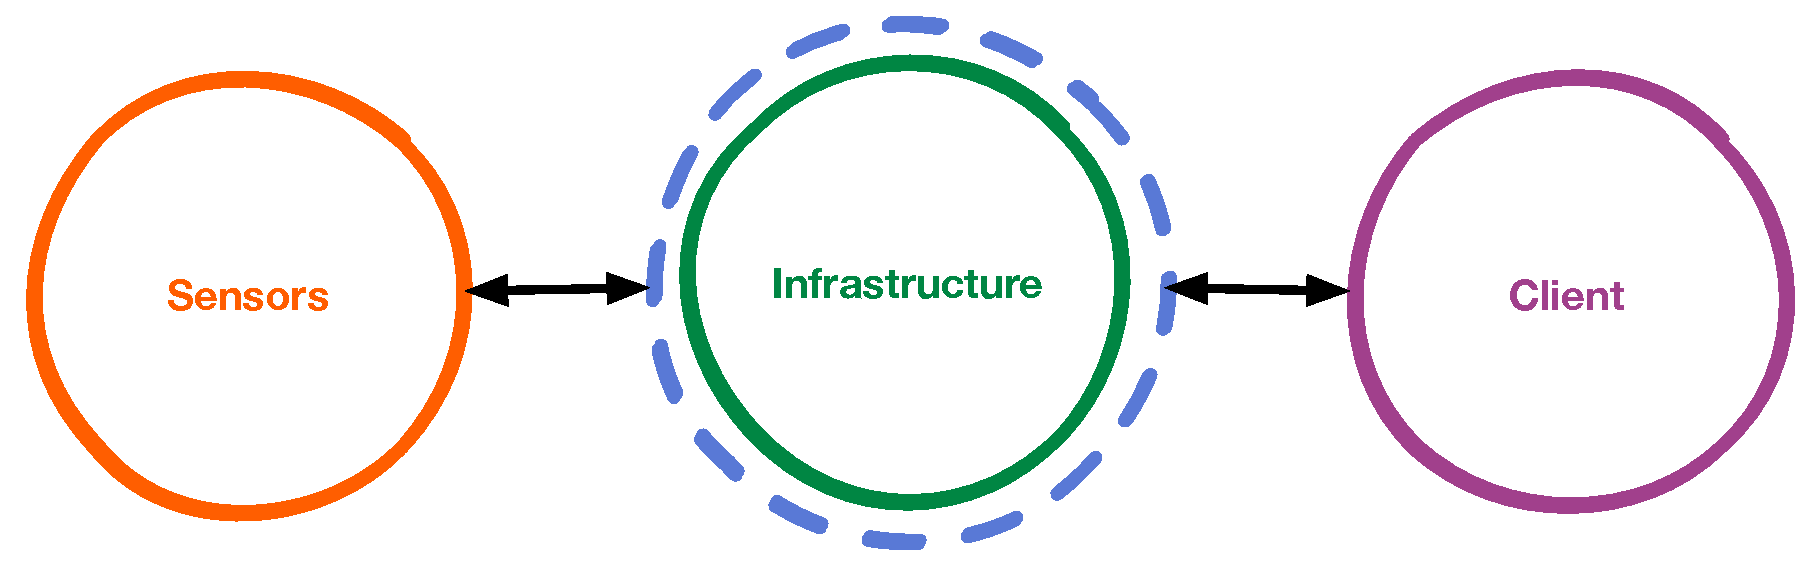
\includegraphics[width=\columnwidth]{figures/system_architecture.pdf}
  \caption{System architecture with communication layer.}
  \label{fig:architecture}
\end{figure}

The next sections will cover each part of the solution in detail.

\subsection{Sensors}
To gather data about the users presence and availability we use sensors.
This project has been restricted to only look at sensors which are available in commodity laptops.
We define a commodity laptop to be a device you can buy at any computer store.
The device should be able to run your operating system of choice.
It should have a camera, an input device, a microphone and radios such as Wi-Fi and Bluetooth built-in.

%TODO check the section and make sure we do what we say here.
In this section we will have a look at some of the sensing capabilities of a commodity laptop.
We will discuss the strengths and weaknesses of these sensors.
As well as providing some reasoning for choosing the sensors we have used in our client.

\subsubsection{Keyboard and Mouse}
By using the mouse and keyboard as sensors we collect every mouse movement and keyboard events and send the last recorded activity every second.
With this information we can infer presence due to the fact that there is someone triggering these events.

The issue with using keyboard and mouse as sensors, is that even though they are a strong indicator of presence, we cannot decipher, based on these two sensors alone, who or what this presence is.
We can tie the machine to a specific user, but we can not infer if the machine is being used by a colleague or if a cat decide to rest on the keyboard.

Another issue with mouse and keyboard sensors is that they provide a very weak indicator of non-presence.
When a key is pressed or the mouse moved, we know that someone is interacting with the machine, but the lack of action cannot tell us whether a user is present or non-present.
A user could be talking on the phone, reading, watching a video etc. all in which the user is present, but the mouse and keyboard cannot provide us with this information.

In terms of interruptibility the information from the mouse and keyboard is too ambiguous to deduct whether a user is busy or interruptible.
If the identity of the user sitting in front of the computer could be confirmed, it would still be difficult to determine whether the behavior is an indication of interruptibility.
An approach to determine interruptibility based on these sensors, would involve sending all information to the decision logic, effectively acting as a key logger, and therefore raising security and privacy issues.
% Jeg ved ikke om det er noget vi skal gå i dybden med, eller om det er nok bare at nævne det her.... eller om det overhoved skal nævnes.
% Min overvejelse er om man kunne bruge en vægtet dictionary hvor specifikke ord fik en vægt på hvor arbejds releterede de er og evt kombinere det med en form for pattern matching hvor sprog mønstre blev undersøgt.
This approach will be described later in the decision logic section.

\subsubsection{Microphone}
The use of a microphone as a sensor allows Approximator to sense the presence of a user, even if the user is not directly interacting with the machine.
With more advanced speech recognition algorithms it could even be used to identify the user/users speaking.
This would provide us not only with presence, but also identity, which was a problem with the keyboard and mouse sensors.

The same issue with the detection of non-presence also appears with the microphone, it is not possible to infer non-presence from the lack of sound.
As described with the keyboard and mouse sensors, a user can perform activities that does not trigger the sensor, and thus be present without detection.

Beside the detection of presence, the microphone provides a tool for inferring interruptibility.
According to Fogarty et al\cite{fogarty2005predicting} speaking present a situation of non-interruptibility.

We have chosen to omit the microphone sensor.
There is a high risk of collecting too much noise compared to the signal we need.
The work environment would need to be very quiet for us to use a normal microphone as a reliable sensor.
For this reason we have dropped the microphone sensor.

\subsubsection{Camera}
Like the microphone the camera enables Approximator to sense the presence of a user without the user having to interact with the machine, but differs in the way it does so.
In the setting of a room a microphone can sense if someone is in the room, but it is hard for the microphone to infer where in this room that they are located.

The camera can sense if someone is directly in front of the screen, which supplies a powerful indicator of presence, as well as an indicator of non-presence.
Unlike the other sensors, the camera can sense if a user is sitting in front of the machine, even if the user is not directly interacting with the machine.
But even though the camera can infer non-presence, there are still some issues.
If a user is located in their office but not visible to the camera, the sensor will report non-presence.

The camera could apply face-recognition in order to determine the identity of the user present.
It could also be used to detect actions that the user is executing e.g. entering the room leaving, leaving the room, reading a book etc. that can be used to measure interruptibility.

\subsubsection{Bluetooth and Wi-Fi}
These radios can detect other devices such as mobile devices or beacons.
If we assume that a user carries his/her mobile device with them, then the Bluetooth or Wi-Fi beacon from their device can be used to infer the users proximity to the machine.
Another usage is if the office the user works in have beacons installed at the workplace, either as Bluetooth or Wi-Fi beacons, then the machine can infer its current symbolic location.
This can be used to infer presence by detecting if the mobile device is nearby.
The issue here is if the user should forget their mobile device, either nearby the machine or at home.
In these cases the sensor would receive false data i.e. data that provides wrongful information regarding presence or interruptibility.
These sensors rely heavily on factors and devices external to the users laptop which makes it more volatile and prone to errors.

\subsubsection{Lightsensor}
The light sensor measures the ambient light of the environment.
This can be used to sense if the laptop is in a dark or light room.
The conclusions that can drawn from this sensor is already provided by the other inputs.
Darkness can be easily detected using the camera.

\subsubsection{Process monitor}
This sensor is slightly different than the others since it primary purpose is not to sense presence, but interruptibility.
The idea of the process monitor is to supply it with a list of processes (programs) running on the users computer that it should monitor.
This list consists both of work and leisure associated processes, and the process monitor report if any and which program are in the foreground. %and receiving user input.
Through this we obtain the same or weaker notion of presence and non-presence as we did with the keyboard and mouse sensor, but gain a stronger tool to infer interruptibility.

\subsubsection{Geo-location}
This sensor works by looking up the machines registered IP address, or if available uses the machines built-in GPS, and uses this to acquire a geographical address.
Knowing the whereabouts of the machine neither infers presence nor interruptibility on its own.
But it does supply the other sensors and the decision module with useful information regarding the geographical setting of the machine.
The most simple use of this is to detect if the machine currently resides at the office, home, or another location.
But one of the more useful appliances would be in combination with the camera.
If the camera can detect action such as a user entering or leaving the room, this information could tells us whether the a user is in close proximity to the machine, but only that.
Combined with even the coarse location of the machine, Approximator could infer that a user was in a specific office, in close proximity the machine.

\subsubsection{Calendar Sensor}
This sensor can look at the users calendar and get information about events entered here.
Events can help identify a users activities during the day, like scheduled meetings or conference calls that would render the user non-interruptible.
Detecting events from a users calendar is strongly coupled with the way the user adds events to his/her calendar.
It could be difficult to infer anything more than presence information which is also available through the camera and the keyboard and mouse.

\subsubsection{Chosen Sensors}
The project scope limits us from using sensors outside of a commodity laptop and from using sensors that requires prior knowledge of the environment or the user. This limitation excludes the Calendar sensor, Geo-location and the Process monitor, as they all require prior knowledge about the user.
The Calendar sensor needs to know which calendar provider the user is using, the Process monitor requires information on which program are work related for the user and Geo-location needs to know to which areas are home, work and otherwise.
The Bluetooth and Wi-Fi are also limited by the scope, since they rely on external beacons to signal position.
The microphone would be a good choice as a sensor, but as most software developers work in shared offices this would generate a significant amount of noise data. 
Therefore we have chosen to omit the microphone.
By using the Camera, Keyboard and Mouse as sensors, we stay within the scope of the project, and still get a good amount of data to infer presence and interruptibility from.
By using the Camera as sensor we can omit the Lightsensor, due to redundancy in sensor features.

Our final choice of sensors are Camera, Keyboard and Mouse.
 
 

\subsection{Infrastructure}
To provide presence and availability information to cloud workers we need a few things.
Firstly we need to gather data input from the working environment.
Secondly we need to aggregate this data and combine it for each user.
Lastly we need to look at the data and through analyzes provide presence and availability information.

All these tasks are combined in our infrastructure which can read input from sensors and analyze this with a decision module.

The work flow of the infrastructure is:
\begin{enumerate}
  \item Gather data
  \item Aggregate data
  \item Analyze data
  \item Provide data
\end{enumerate}

\subsubsection{Design}
The infrastructure is built to support many sensors for each user.
This modelling can lead to a very high amount of sensors connecting to the system.
To support this scalability need we base our system on the actor model by Carl Hewitt \cite{hewitt1973universal}.

Many software applications are written using the object oriented modelling.
The actor model is an alternative way to model computer programs.
In the actor model the unit of work is an actor.
In object oriented programming the unit of work is an object.
Actors communicate by sending messages to each other.
Actors does not share state, making it possible to run actors in parallel and even on different machines.
This makes the actor model a good candidate for building highly scalable applications.

There are several frameworks implementing the actor model, such as Akka \cite{akka}, Project Orleans \cite{orleans} and most famously Erlang \cite{erlang}.
For this project we have chosen Akka because it is Java based.
This supports the technical knowledge in our group.

We use the general programming language Scala \cite{scala} to program our Akka-based infrastructure.


\begin{figure}[H]
  \centering
  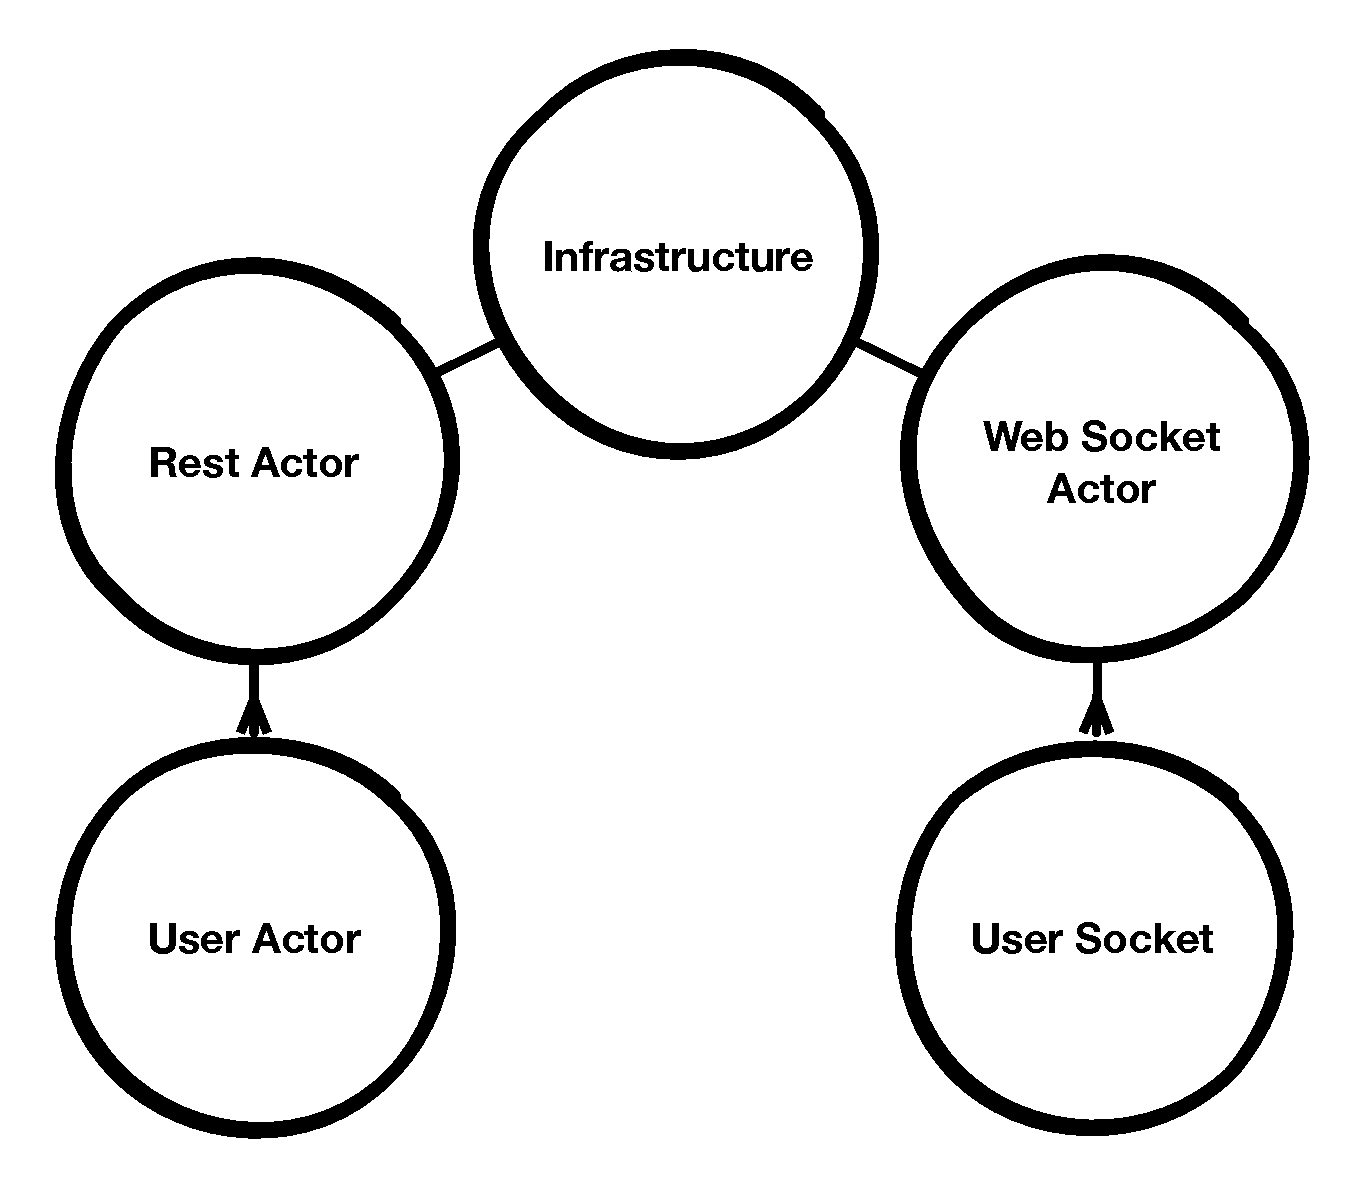
\includegraphics[width=\columnwidth]{figures/infrastructure_design.pdf}
  \caption{Infrastructure Design.}
  \label{fig:infrastructure}
\end{figure}

It is possible to deploy Akka applications on a server which can run Java.
For this project we have chosen to deploy our system to Azure \cite{azure}, Microsoft's cloud service for developers.
Having the infrastructure running at a cloud provider makes it reachable from the standard internet.
This enables us to build sensors and demonstrators that can run anywhere, as long as they have an internet connection they can reach our infrastructure.

\subsubsection{Data}
Gathering data happens by sensors providing data.
To communicate with our infrastructure a sensor needs to register with the service.
When a sensor registers itself it provides a username.
This username is used to aggregate a group of sensors together around the notion of user.

\subsection{Client}
Windows based user installable application.
The sensor actually combines two parts of the system.
The sensors are built into the client.
This is done for easy of use for the end user.
Merging the two parts makes it possible to get both parts on the users laptop with a single installation.

\subsubsection{Ease of deployment}
We have focused on creating an easy to deploy system.
The infrastructure component can be deployed to any server capable of running the Java Virtual Machine (JVM).
Currently it is possible to get the source code from GitHub\footnote{\url{https://github.com/mofus/GSE/tree/master/Server}}.
The source code requires that Java and SBT is installed.
With the source code on the server it is a simple run command which will compile, fetch dependencies and run the infrastructure.

The client is even easier this is currently a Windows application which can be downloaded and run directly on any newer Windows installation.

The clients source code is available in our GitHub repository.
The client was written with the .NET framework which makes it easy to build the client on other platform with the Mono compiler.

\section{Decision Logic}
\label{sec:decision_logic}
We want to identify a software engineer’s interruptibility value using the sensors in a laptop.
To achieve this there are three sensors providing data; keyboard, mouse and camera (face detection).

Raw sensor data does not say much about presence or availability.
The captured sensor data must be analyzed in order to make sense of it.
The infrastructure has a decision module which can calculate interruptibility values from the sensor inputs.

\subsection{Building a model}
A manual classification approach has been used to classify the collected data.
Two test subjects, user A and user B, was recorded in their work environment.
User A showed a clear coalition between patterns in the sensor data and the reported interruptibility.
Three major scenarios was identified by looking at the data, they are listed in Figure~\ref{fig:scenarios}.

\begin{figure}[H]
  \centering
      \begin{tabular}{@{}llll@{}}
      \toprule
      \textbf{Scenario} & \textbf{1} & \textbf{2} & \textbf{3}      \\ \midrule
      Interruptible     & No         & No         & Yes             \\
      Primary sensor    & Camera     & Keyboard   & Mouse           \\
      Example task 1    & Reading    & Writing    & Browsing        \\
      Example task 2    & Video Chat & Coding     & Switching tasks \\ \bottomrule
      \end{tabular}
  \caption{The three identified scenarios.}
  \label{fig:scenarios}
\end{figure}

User B however did not show any clear indication of patterns that could identify a given scenario.
This could be because software engineers work in different ways.
There is also a chance that user B is an outlier and therefore not representing the generic software engineer.
Then again it could also be that it is user A who is an outlier, we do not know.
It would have been much more clear if any of these theories was true if more test subjects had been involved.

\subsection{Scenario detection}
We use a centralized algorithm to detect which scenario the user is in.
The algorithm is running on the infrastructure server.
Here it constantly looks at a moving window of incoming sensor data.
The window is 30 seconds long and contains all the sensor data from this period.
The algorithm is shown in Figure~\ref{fig:decision_logic}.

\begin{figure}[H]
  \centering
  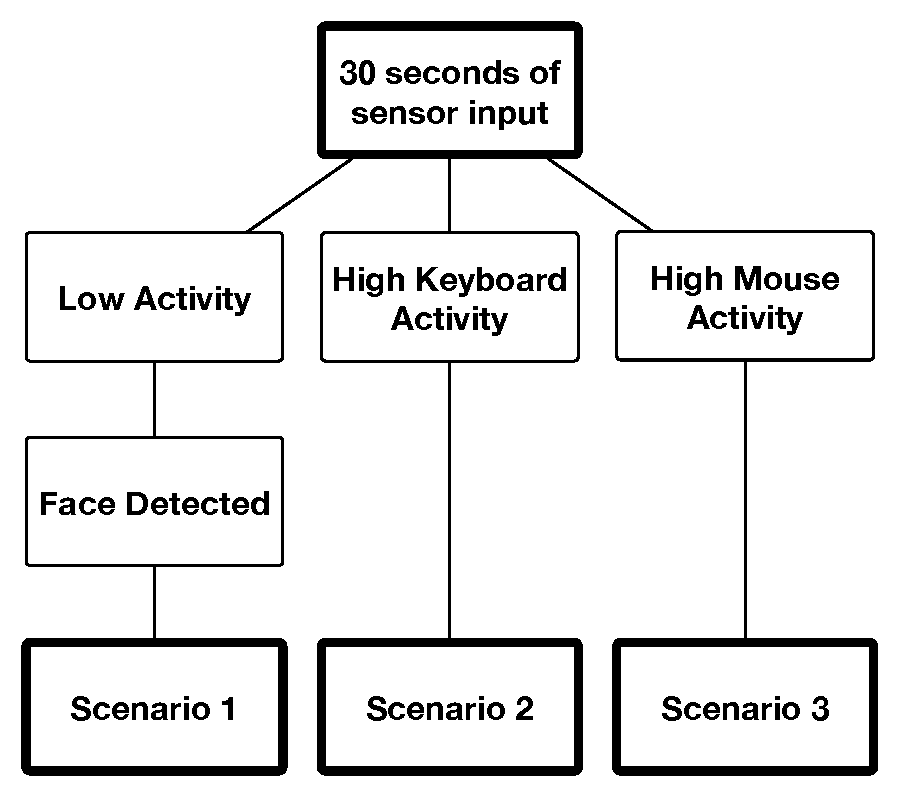
\includegraphics[width=\columnwidth]{figures/decision_logic.pdf}
  \caption{Decision logic for detecting scenarios.}
  \label{fig:decision_logic}
\end{figure}

\textbf{Scenario 1} is detected using face detection.
If a user is sitting in front of the computer the face detection will detect the user as being present.
Detection happens with a frontal or profile detection depending on the angle the camera sees the users face.

We try to catch the scenario of a user sitting in front of the computer using it without the mouse and keyboard as main input.
This could be because the user is reading, having a conversation or something similar.

The keyboard sensor identifies \textbf{scenario 2}.
When a user is typing away, it is interpreted as the user is concentrating on work.
This work can be writing, coding or other keyboard heavy tasks.

When a user is moving the mouse a lot, we identify it as \textbf{scenario 3}.
We hypothesize that heavy mouse activity is an indicator for casual activity.
This could be browsing, moving files or simply a switch of context between work sessions.


\section{Evaluation}
In order to compare the performance of Approximator to the result from Forgartys study, the same method for evaluation is followed during the experiments in this paper.

\subsection{Method}
\label{method}
The experiment was conducted in two stages.
First the two test subjects are recorded in their work environment with a camera, while Approximators sensors collected data.
The second stage was conducted by inviting people from the software development community to do a survey where they reviewed the experiment.
At the survey the participants were asked to assess interruptibility for the two test users based on short sequences of video, showing the test users in random selected situations in their work environment.

\subsubsection{Stage One}
The two male test subjects were 25 and 34 years of age.
The first test subject worked for a security company where his primary task was to maintain and develop on the company system.
Since the company also have offices in other countries, this test subject often did parallel development with the out-of-country teams.
He worked in shared offices, where he shared the office with 3-4 other employees, often people assigned to the same project or with a similar skillset.
It was possible to close the door to these offices, but that rarely occurred.

The second test subject worked for a software company where his primary task was to develop server solutions.
The company has offices in several locations, including home offices.
Our test subject worked in a home office, placed in the basement of his house.
All communication with colleges happens online, either through instant messaging or audio chats.

The test subjects was recorded with a Sony Handycam HDR-CX360 with wide angle lens and was recorded in mp4 with 720x576 format at 25 frames per second.
The original recording was recorded with sound, but the sound was removed for the test.
The camera was placed at an angle that did not allow for the content of their screen to be visible.
The angle did however show as much of the office as possible, while showing the face of the test subject.

\begin{figure}
  \centering
  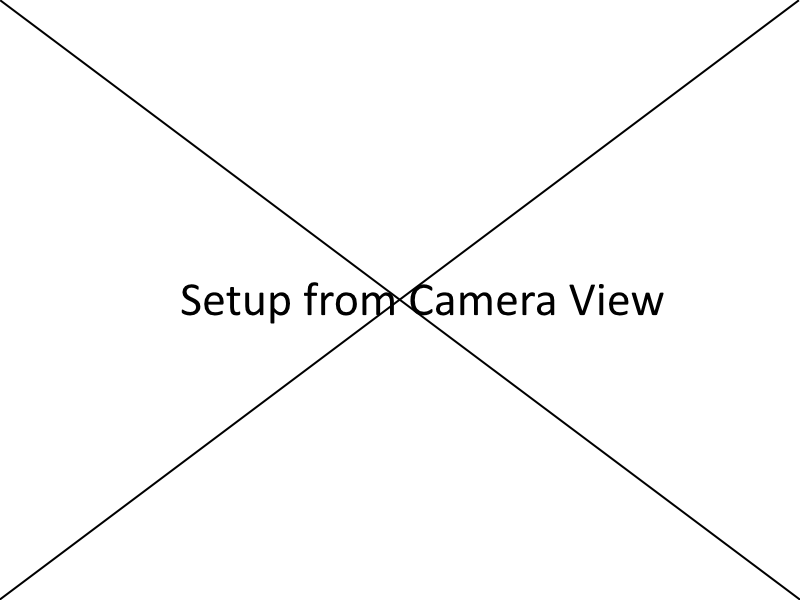
\includegraphics[width=\columnwidth]{figures/experiment_setup.png}
  \caption{View of experiment setup.}
  \label{fig:experiment}
\end{figure}

Approximator was running on a Lenovo T440s Intel Core i5 64-bit processer 8GB RAM with a Windows 7 OS and a Microsoft Surface Pro 3 i5 processer 8GB Ram with Windows 8.1 OS.
Both machines was mounted in an office dock setup connecting the machine to an external screen, keyboard and mouse.
Approximator utilized the keyboard, mouse and camera as sensors, and sent data from these sensors to the infrastructure throughout the experiment.
This data was to used later in our process.
Approximator was specially configured to prompt a visual and audio bell for the test subject at random intervals averaging at two times per hour.
The test subjects were instructed to self-report their own level of interruptibility on a scale of 1 (Highly Interruptible) to 5 (Highly Non-Interruptible) by show of fingers on one hand when prompted.
The test subjects had no way of pausing the application, but could request retroactively to have sequence deleted if necessary.
The prompts where the test subjects was not present was removed from the dataset after the experiment.
If it should happen that the test subjects clearly registered the prompt, but did not signal their interruptibility, due to them being on the phone or engaged in a other activity that required their full attention, then these would be interpreted by us as a highly non-interruptible events.

The experiment was conducted over a period of two workdays from 9 am to 4:30 pm, yielding a total of 30 hours of video and 43 prompts.

\subsubsection{Stage Two}
\label{stage_two}
At this stage an application with the explicit purpose of peer reviewing the collected recordings was created.
People from the software development community were invited to partake in the survey, and did so under supervision from two of the researchers.

When the estimator subjects started the survey, they were asked to rate each video on a scale of 1 (Highly Interruptible) to 5 (Highly Non-Interruptible).
They where informed that they should act as though they where colleges with the video subject.
And finally that they should ask the researchers if they had any questions.
Afterwards they were required to enter their demographic information.
These demographical questions consisted of gender, age, and ethnicity.
The demographic distribution is provided since it may affect peoples ability to interpret interruptibility,

\begin{figure}
  \centering
  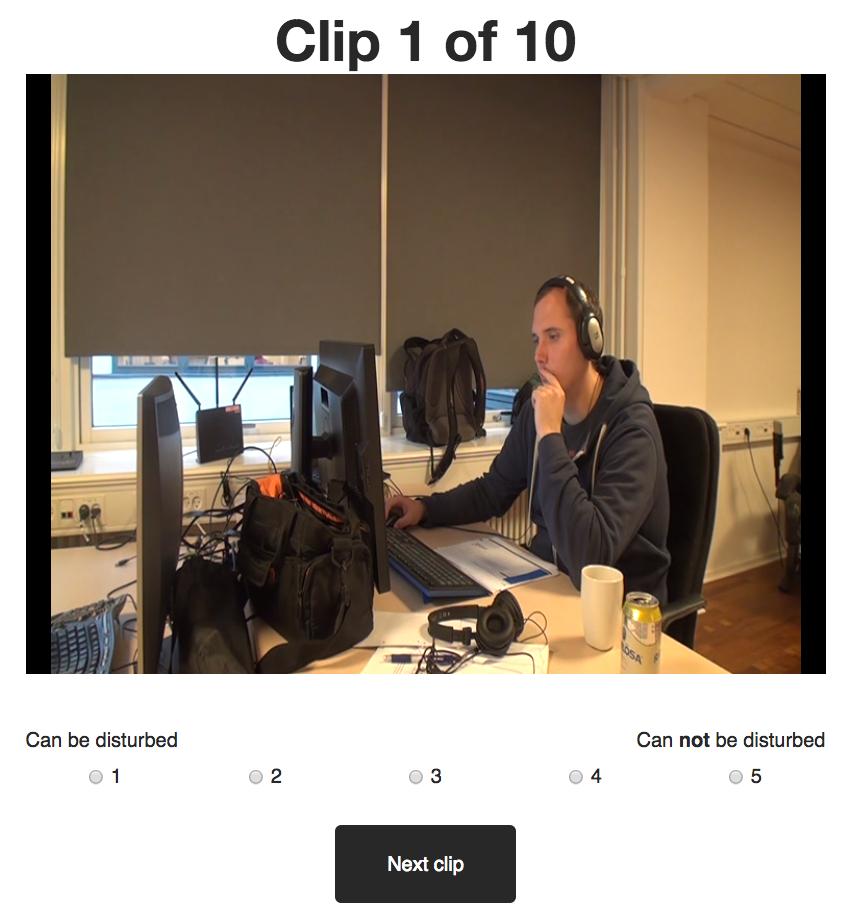
\includegraphics[width=\columnwidth]{figures/webpage_screenshot.png}
  \caption{Screenshot of survey webpage.}
  \label{fig:webpage}
\end{figure}

The content survey consists of 5 unique sets with 7 different video clips from the first stage of the experiment.

Each clip contained the last 30 seconds leading up to the video subject being prompted for self-report.

Each estimator subject was shown one of the 5 different sets of video with 3 random repetitions from the same set.
The 3 random repetition is to ensure that the estimator is confident about their answer.
If more than two repetitions deviated more than two points compared to the original answer, the results from that estimator subject was deemed invalid.
The estimator could replay the sequence as many times as they wanted until they felt they could give a valid assessment.
Each sequence was played in full length before the user could rate it and proceed to the next.

\subsection{Data analysis}
After the experiment was concluded, the results gathered from Approximator was compared to the test persons, and the users.
This was done by plotting the values into two confusion matrices.
One comparing the answers of user to answers of the test users.
And one comparing the answers of the user to the results of Approximator.
By finding correlations between hits in the test-user/user and Approximator/user results, we could compare how Approximator performs in relation to human judgement, and also compare our findings to those found by Fogarty et al \cite{fogarty2005predicting}

\subsection{Results}
In this section we will go over our results that we have collected through the experiments mentioned in \autoref{sec:method}.
This section is divided into the results collected from the review group, and the results collected from Approximator.

\subsubsection{Review Group Results}
Out of the 43 prompts, 35 was used for the review test.
The remaining 8 was not applicable since the test subject was not present at the time of the prompt.

\begin{figure}
  \centering
  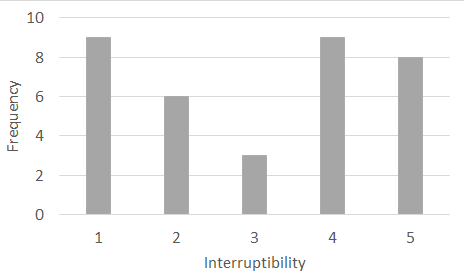
\includegraphics[width=\columnwidth]{figures/Interruptibility_values_videotest.png}
  \caption{Frequency of interruptibility values reported by the test subjects, ranging from 1 (Highly Interruptible) to 5 (Highly Non-Interruptible).}
  \label{fig:interruptibilityFrequency}
\end{figure}

A total of 19 people participated in the survey.
The video clip sets A, B, C and D were surveyed by 4 people while set E was surveyed by 3 people.
All surveys were valid and consistent answers.
Our dataset has a mean of 2.77, median of 3, mode of 3, range of 4 and a standard deviation of 1.288.

Although answers were consistent and participants clearly understood the task, the accuracy of the participants were overall poor.
As shown in \autoref{tab:survey_accuracy} the average precision among all sets were around 28\%.
We attribute this low score to the fact that is very hard to precisely rate another persons interruptibility on a scale from 1 to 5.
In order to account for this we use the same scale conversion as Fogarty\cite{fogarty2005predicting}.
But unlike Fogarty who did the scale conversion, by converting all values from 1-4 as 1 and 5 as 5, we did it as followed.
For all answers in the survey we change values of 1-3 to be 1 and 4-5 to be 5.
This gives us a more binary representation of interpretation of the data.
As shown in \autoref{tab:survey_accuracy} that yields a much improved average accuracy of 63\%.
The reason that we converted the data differently from Fogarty, lies in Fogartys reason for converting the data in the first place.
Fogartys data showed that the estimator subjects had a tendency to rate the video subjects interruptibility lower than the self-reported value.
Our data shows that there is an even distribution between lower and higher rated values.

When all the data was acquired, we compared the result from the review group to the results from the video experiment.
This was done in a confusion matrix shown in \autoref{tab:video_to_estimator_matrix} and this matrix shows that the overall accuracy lies at 30.08\%, and the accuracy within one is at 62.41\%.
This shows that our review group was about as accurate as Forgarty review group \cite{fogarty2005predicting} that achieved an overall accuracy of 30.7\% and a within one accuracy of 65.8\%.

As discussed in \nameref{stage_two} the demography of the participants could impact the interpreted interruptibility of other people.
\autoref{fig:demography_country} shows the distribution of participants by country of origin, \autoref{fig:demography_age} by age and \autoref{fig:demography_gender} by gender.

%Estimator comparison
\begin{table}[h]
  \begin{tabular}{c | c c c c c c}
		\multicolumn{1}{c}{} & & \multicolumn{5}{c}{Estimator Subject Value} \\ \cline{3-7}
		\multicolumn{1}{c}{} & & 1 & 2 & 3 & 4 & 5 \\
		\multirow{5}{*}{\rotatebox[origin=c]{90}{Video Subject Value}}
		& 1	    & \specialcell{12 \\ 9.02\% \\ |}    & \specialcell{9 \\ 6.77\% \\ |}    & \specialcell{11 \\ 8.27\% \\ |}   & \specialcell{3 \\ 2.26\% \\ |}    & \specialcell{0 \\ 0\% \\ |}\\
		& 2		& \specialcell{4 \\ 3.01\% \\ |}     & \specialcell{6 \\ 4.51\% \\ |}    & \specialcell{8 \\ 6.02\% \\ |}    & \specialcell{5 \\ 3.76\% \\ |}    & \specialcell{1 \\ 0.75\% \\ |}\\
		& 3		& \specialcell{3 \\ 2.26\% \\ |}     & \specialcell{0 \\ 0\% \\ |}       & \specialcell{4 \\ 3.01\% \\ |}    & \specialcell{3 \\ 2.26\% \\ |}    & \specialcell{2 \\ 1.50\% \\ |}\\
		& 4		& \specialcell{4 \\ 3.01\% \\ |}     & \specialcell{5 \\ 3.76\% \\ |}    & \specialcell{9 \\ 6.77\% \\ |}    & \specialcell{12 \\ 9.02\% \\ |}   & \specialcell{4 \\ 3.01\% \\ |}\\
        & 5		& \specialcell{7 \\ 5.26\% \\ |}	& \specialcell{5 \\ 3.76\% \\ |}     & \specialcell{4 \\ 3.01\% \\ |}    & \specialcell{6 \\ 4.51\% \\ |}    & \specialcell{6 \\ 4.51\% \\ |}
  \end{tabular}
  \caption{Confusion matrix comparing the estimator subject values to the values of the video subject. \\Overall Accuracy: 30.08\% Accuracy Within 1: 62.41\%}
  \label{tab:video_to_estimator_matrix}
\end{table}

\begin{table}[h]
  \begin{tabular}{c | c c c}
		\multicolumn{1}{c}{} & & \multicolumn{2}{c}{Estimator Subject Value} \\ \cline{3-4}
		\multicolumn{1}{c}{} & & 1 & 5 \\
		\multirow{5}{*}{\rotatebox[origin=c]{90}{Video Subject}}
		& 1	    & \specialcell{57 \\ 42.86\% \\ |}    & \specialcell{14 \\ 10.53\% \\ |}\\
		& 5		& \specialcell{34 \\ 25.56\% \\ |}     & \specialcell{28 \\ 21.05\% \\ | }
  \end{tabular}
  \caption{Reduced confusion matrix comparing the estimator subject values to the values of the video subject. \\Overall Accuracy: 63.91\%}
  \label{tab:reduced_video_to_estimator_matrix}
\end{table}

\subsubsection{Approximator Results}
The sensors from Approximator collected data throughout the 30 hours of the experiment resulting in a total collection of 86823 mouse events, 16151 face detection events and 28629 keyboard events.
In our experiment, we only took the events that could be compared to the video subjects self-reports into account, so the data collected 30 seconds before the video subject was prompted.
The distribution of these events can be found in \autoref{tab:event_distribution}.

\begin{table}[h]
  \begin{tabular}{@{}lll@{}}
    \toprule
     & Video subject 1 & Video subject 2\\ \midrule
    Mouse events       & 984    & 534    \\
    Keyboard events       & 319    & 218    \\
    Face detection events       & 244    & 113    \\ \midrule
    Total   & 1547 & 865\\ \bottomrule
  \end{tabular}
  \caption{Distribution of events collected by Approximator divided over the Video subjects}
  \label{tab:event_distribution}
\end{table}

This data was used by the decision module to produce interruptibility values based on the interruptibility model mentioned in \nameref{method}.
We compared the data produced from Approximator with the values reported by the video subject the same way as we compared the estimator subjects values with those of the video subjects, see \autoref{tab:video_to_approximator_matrix}.

The overall accuracy of Approximator was 31.43\% making it slightly more accurate than the estimator subjects assessments by 1.35\%.
If we look at the reduced matrices \autoref{tab:reduced_video_to_estimator_matrix} and \autoref{tab:reduced_video_to_approximator_matrix}, we see that the overall accuracy from the estimators are 1.05\% better than Approximators accuracy.
This seemed fairly odd to us, so we took a closer look at the interruptibility values produced by Approximator.
The investigation showed that video subject 2 values was very accurate with an overall accuracy of 41.67\% with a within one accuracy of 91.67\%.
But the investigation also showed that the values for video subject 1 was all ones (highly-non-interruptible).

The reason for this strange abnormality can be pinned down to 5 possible reasons
\begin{enumerate}
  \item The reedings are correct, and video subject 1 was prompted when at interruptibility value 1.
  \item Video subject 1 did not do much work during the 2 days of recording, but did not want that to appear on the results.
  \item The sensor units were in some way faulty.
  \item The decision module was in some way faulty.
  \item The decision module's interruptibility model does not support video subject 1 tasks as work.
\end{enumerate}
We can exclude 1 due to the self-report stating otherwise.
Reason 2 seems unlikely due to review groups assessment was more accurate on video subject 1 than on video subject 2.
Reason 3 can be excluded due to \autoref{tab:event_distribution} shows that there is plenty of sensor input on all sensor channels.
Reason 4 is also unlikely since the data of video subject 1 and video subject 2 was processed by the same module, and there was no modifications to the module in between processing.
Reason 5 is the most likely since the interruptibility model, \autoref{fig:scenarios} relies heavy on keyboard input to infer non-interruptibility and mouse events to infer interruptibility. \autoref{tab:event_distribution} shows that that video subject 1 have an approximately 1:3 ratio of keyboard vs mouse events, whereas video subject 2 have an approximately 1:2 ratio of keyboard vs mouse events.
This gives an indication that video subject 1 work tasks are more mouse based than those of video subject 2.


%Approximator comparison
\begin{table}[h]
  \begin{tabular}{c | c c c c c c}
		\multicolumn{1}{c}{} & & \multicolumn{5}{c}{Approximator Value} \\ \cline{3-7}
		\multicolumn{1}{c}{} & & 1 & 2 & 3 & 4 & 5 \\
		\multirow{5}{*}{\rotatebox[origin=c]{90}{Video Subject Value}}
		& 1	    & \specialcell{8 \\ 22.86\% \\ |}    & \specialcell{1 \\ 2.86\% \\ |}    & \specialcell{0 \\ 0\% \\ |}   & \specialcell{0 \\ 0\% \\ |}    & \specialcell{0 \\ 0\% \\ |}\\
		& 2		& \specialcell{5 \\ 14.29\% \\ |}     & \specialcell{0 \\ 0\% \\ |}    & \specialcell{1 \\ 2.86\% \\ |}    & \specialcell{0 \\ 0\% \\ |}    & \specialcell{0 \\ 0\% \\ |}\\
		& 3		& \specialcell{2 \\ 5.71\% \\ |}     & \specialcell{0 \\ 0\% \\ |}       & \specialcell{0 \\ 0\% \\ |}    & \specialcell{1 \\ 2.86\% \\ |}    & \specialcell{0 \\ 0\% \\ |}\\
		& 4		& \specialcell{6 \\ 17.14\% \\ |}     & \specialcell{0 \\ 0\% \\ |}    & \specialcell{1 \\ 2.86\% \\ |}    & \specialcell{1 \\ 2.86\% \\ |}   & \specialcell{1 \\ 2.86\% \\ |}\\
        & 5		& \specialcell{5 \\ 0\% \\ |}	& \specialcell{0 \\ 0\% \\ |}     & \specialcell{0 \\ 0\% \\ |}    & \specialcell{1 \\ 2.86\% \\ |}    & \specialcell{2 \\ 5.71\% \\ |}
  \end{tabular}
  \caption{Confusion matrix comparing the values produced by Approximator to the values of the video subject. \\Overall Accuracy: 31.43\% Accuracy Within 1: 62.86\%}
  \label{tab:video_to_approximator_matrix}
\end{table}

\begin{table}[h]
  \begin{tabular}{c | c c c}
		\multicolumn{1}{c}{} & & \multicolumn{2}{c}{Approximator Value} \\ \cline{3-4}
		\multicolumn{1}{c}{} & & 1 & 5 \\
		\multirow{5}{*}{\rotatebox[origin=c]{90}{Video Subject}}
		& 1	    & \specialcell{17 \\ 48.57\% \\ |}    & \specialcell{1 \\ 2.86\% \\ |}\\
		& 5		& \specialcell{12 \\ 34.29\% \\ |}     & \specialcell{5 \\ 14.29\% \\ | }
  \end{tabular}
  \caption{Reduced confusion matrix comparing the values produced by Approximator to the values of the video subject. \\Overall Accuracy: 62.86\%}
  \label{tab:reduced_video_to_approximator_matrix}
\end{table}

%Anders data only
\begin{table}[h]
  \begin{tabular}{c | c c c c c c}
		\multicolumn{1}{c}{} & & \multicolumn{5}{c}{Approximator Value} \\ \cline{3-7}
		\multicolumn{1}{c}{} & & 1 & 2 & 3 & 4 & 5 \\
		\multirow{5}{*}{\rotatebox[origin=c]{90}{Video Subject Value}}
		& 1	    & \specialcell{2 \\ 16.67\% \\ |}    & \specialcell{1 \\ 8.33\% \\ |}    & \specialcell{0 \\ 0\% \\ |}   & \specialcell{0 \\ 0\% \\ |}    & \specialcell{0 \\ 0\% \\ |}\\
		& 2		& \specialcell{0 \\ 0\% \\ |}     & \specialcell{0 \\ 0\% \\ |}    & \specialcell{1 \\ 8.33\% \\ |}    & \specialcell{0 \\ 0\% \\ |}    & \specialcell{0 \\ 0\% \\ |}\\
		& 3		& \specialcell{1 \\ 8.33\% \\ |}     & \specialcell{0 \\ 0\% \\ |}       & \specialcell{0 \\ 0\% \\ |}    & \specialcell{1 \\ 8.33\% \\ |}    & \specialcell{0 \\ 0\% \\ |}\\
		& 4		& \specialcell{0 \\ 0\% \\ |}     & \specialcell{0 \\ 0\% \\ |}    & \specialcell{1 \\ 8.33\% \\ |}    & \specialcell{1 \\ 8.33\% \\ |}   & \specialcell{1 \\ 8.33\% \\ |}\\
        & 5		& \specialcell{5 \\ 0\% \\ |}	& \specialcell{0 \\ 0\% \\ |}     & \specialcell{0 \\ 0\% \\ |}    & \specialcell{1 \\ 8.33\% \\ |}    & \specialcell{2 \\ 16.67\% \\ |}
  \end{tabular}
  \caption{Confusion matrix comparing a subset of values produced by Approximator to the values of the video subject. \\Overall Accuracy: 41.67\% Accuracy Within 1: 91.67\%}
  \label{tab:subset_video_to_approximator_matrix}
\end{table}

\begin{table}[h]
  \centering
  \begin{tabular}{@{}lll@{}}
    \toprule
    Test Set     & Adjusted & Original \\ \midrule
    A       & 50.99\%    & 21.42\%    \\
    B       & 57.14\%    & 21.42\%    \\
    C       & 82.14\%    & 39.28\%    \\
    D       & 78.57\%    & 32.14\%    \\
    E       & 47.61\%    & 28.57\%    \\ \midrule
    Average & 63.09\%    & 28.57\%    \\ \bottomrule
  \end{tabular}
  \caption{Accuracy of survey participants interpreting test subjects interruptibility}
  \label{tab:survey_accuracy}
\end{table}

\begin{figure}[ht]
  \centering
  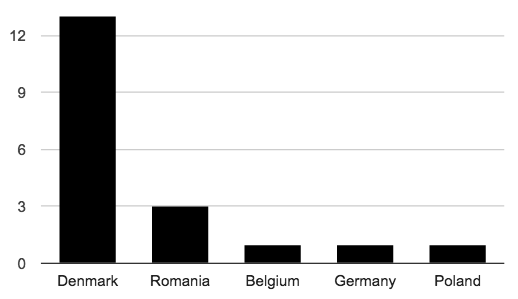
\includegraphics[width=\columnwidth]{figures/demography_country.png}
  \caption{Demography of survey participants by Country of origin}
  \label{fig:demography_country}
\end{figure}

\begin{figure}[ht]
  \centering
  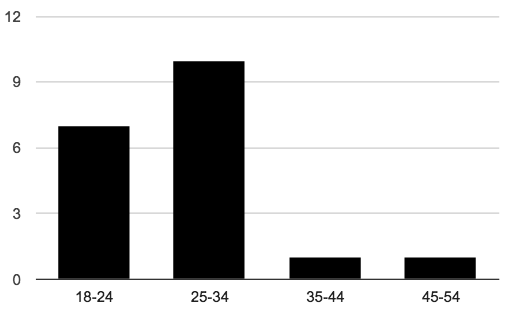
\includegraphics[width=\columnwidth]{figures/demography_age.png}
  \caption{Demography of survey participants by Age range}
  \label{fig:demography_age}
\end{figure}

\begin{figure}[ht]
  \centering
  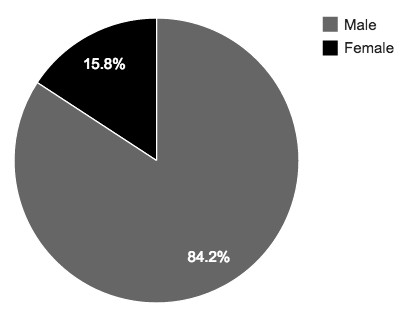
\includegraphics[width=\columnwidth]{figures/demography_gender.png}
  \caption{Demography of survey participants by Gender}
  \label{fig:demography_gender}
\end{figure}


\section{Discussion}

% Better ways to do experiment
%   Asking test subjects to provide their assesed interruptibility might interrupt them

Many factors affect how people asses human interruptibility as noted in \cite{Avrahami2007}.
These aspects are hard to incorporate in prediction models.
In this paper we use a limited demography of people to asses interruptiblity.
Factors like culture, age and ethnicity may significantly impact the results.

This paper bases its research background and evalutation of the work done in \cite{fogarty2005predicting} but has a number of different factors. This paper and \cite{fogarty2005predicting} are written over 10 years apart. \cite{fogarty2005predicting} relied heavily on factores like closed office doors and talking on the phone. Today open office spaces with are much more common than in 2003 and talking on the phone is less common in favor of other means of communication like email, and chat. More notably \cite{fogarty2005predicting} based their studies on knowledge workers in an University administration department while we based our paper on software developers in a CSCW setting.

We had hoped that both our test subjects would show the same coalition in their data.
This was unfortunately not the case.
If a similar project is to succeed, we need a better algorithm for detecting patterns.
Instead of having a centralized generic algorithm we could have learning algorithms on each users’ machine.
An algorithm which could be tailored directly at a given users’ needs would be preferable.
One approach is to construct an algorithm with a learning period.
In the learning period, the user needs to answer interruptibility questions at random intervals.
This way the algorithm could build up some training data to use for future evaluations.

The current sensors only give vague clues to a persons context, through the level of activity.
Additional sensors that could give input about the context, especially in combination with a learning algorithm, could improve our results.
Sensors that could give specific clues to the context about how subject was working e.g. advanced gaze tracking, speech detection, posture detection, desktop monitor, process monitor etc..
Sensors like these would allow for more detailed and less ambiguous interruptibility models, and thereby better accuracy.


\subsection{Future Work}
We chose to focus our paper on the sensors available in a modern laptop for the ease of use and deployability.
Most people today also carry smart phones and newer devices such as fitness trackers and smart watches are gaining popularity.
These devices could supply additional useful data to our infrastructure to enhance the prediction of interruptibility by providing more finegrained position and movement.
We leave these devices for future work as they constrain deployability and are not all common case.

\section{Conclusion}
We set out believing that it was possible to detect a software engineer’s interruptibility value using only the sensors in a laptop.
It turned out that it was possible for one of our two test subjects.
This finding opens more questions than it answers. Is our approach still valid have we tested on more subjects?

We conclude that our initial idea is valid.
However, our project did not include enough test subjects to say anything definite about the feasibility across all software engineers.

\section{Acknowledgements}
We would like to thank Paolo Tell for supervising and guiding us throughout the project.
We are also grateful for the great feedback from Thomas Olof Pederson and Shahram Jalaliniya.
Lastly, we would like to thank all the people who helped do our evaluation.

\balance
\bibliographystyle{acm-sigchi}
\bibliography{ubicomp}

\end{document}
